\documentclass[]{book}
\usepackage{lmodern}
\usepackage{amssymb,amsmath}
\usepackage{ifxetex,ifluatex}
\usepackage{fixltx2e} % provides \textsubscript
\ifnum 0\ifxetex 1\fi\ifluatex 1\fi=0 % if pdftex
  \usepackage[T1]{fontenc}
  \usepackage[utf8]{inputenc}
\else % if luatex or xelatex
  \ifxetex
    \usepackage{mathspec}
  \else
    \usepackage{fontspec}
  \fi
  \defaultfontfeatures{Ligatures=TeX,Scale=MatchLowercase}
\fi
% use upquote if available, for straight quotes in verbatim environments
\IfFileExists{upquote.sty}{\usepackage{upquote}}{}
% use microtype if available
\IfFileExists{microtype.sty}{%
\usepackage{microtype}
\UseMicrotypeSet[protrusion]{basicmath} % disable protrusion for tt fonts
}{}
\usepackage{hyperref}
\hypersetup{unicode=true,
            pdftitle={Medidas de Alpha Diversidad},
            pdfauthor={Carlos Iván Espinosa},
            pdfborder={0 0 0},
            breaklinks=true}
\urlstyle{same}  % don't use monospace font for urls
\usepackage{natbib}
\bibliographystyle{apalike}
\usepackage{color}
\usepackage{fancyvrb}
\newcommand{\VerbBar}{|}
\newcommand{\VERB}{\Verb[commandchars=\\\{\}]}
\DefineVerbatimEnvironment{Highlighting}{Verbatim}{commandchars=\\\{\}}
% Add ',fontsize=\small' for more characters per line
\usepackage{framed}
\definecolor{shadecolor}{RGB}{248,248,248}
\newenvironment{Shaded}{\begin{snugshade}}{\end{snugshade}}
\newcommand{\KeywordTok}[1]{\textcolor[rgb]{0.13,0.29,0.53}{\textbf{{#1}}}}
\newcommand{\DataTypeTok}[1]{\textcolor[rgb]{0.13,0.29,0.53}{{#1}}}
\newcommand{\DecValTok}[1]{\textcolor[rgb]{0.00,0.00,0.81}{{#1}}}
\newcommand{\BaseNTok}[1]{\textcolor[rgb]{0.00,0.00,0.81}{{#1}}}
\newcommand{\FloatTok}[1]{\textcolor[rgb]{0.00,0.00,0.81}{{#1}}}
\newcommand{\ConstantTok}[1]{\textcolor[rgb]{0.00,0.00,0.00}{{#1}}}
\newcommand{\CharTok}[1]{\textcolor[rgb]{0.31,0.60,0.02}{{#1}}}
\newcommand{\SpecialCharTok}[1]{\textcolor[rgb]{0.00,0.00,0.00}{{#1}}}
\newcommand{\StringTok}[1]{\textcolor[rgb]{0.31,0.60,0.02}{{#1}}}
\newcommand{\VerbatimStringTok}[1]{\textcolor[rgb]{0.31,0.60,0.02}{{#1}}}
\newcommand{\SpecialStringTok}[1]{\textcolor[rgb]{0.31,0.60,0.02}{{#1}}}
\newcommand{\ImportTok}[1]{{#1}}
\newcommand{\CommentTok}[1]{\textcolor[rgb]{0.56,0.35,0.01}{\textit{{#1}}}}
\newcommand{\DocumentationTok}[1]{\textcolor[rgb]{0.56,0.35,0.01}{\textbf{\textit{{#1}}}}}
\newcommand{\AnnotationTok}[1]{\textcolor[rgb]{0.56,0.35,0.01}{\textbf{\textit{{#1}}}}}
\newcommand{\CommentVarTok}[1]{\textcolor[rgb]{0.56,0.35,0.01}{\textbf{\textit{{#1}}}}}
\newcommand{\OtherTok}[1]{\textcolor[rgb]{0.56,0.35,0.01}{{#1}}}
\newcommand{\FunctionTok}[1]{\textcolor[rgb]{0.00,0.00,0.00}{{#1}}}
\newcommand{\VariableTok}[1]{\textcolor[rgb]{0.00,0.00,0.00}{{#1}}}
\newcommand{\ControlFlowTok}[1]{\textcolor[rgb]{0.13,0.29,0.53}{\textbf{{#1}}}}
\newcommand{\OperatorTok}[1]{\textcolor[rgb]{0.81,0.36,0.00}{\textbf{{#1}}}}
\newcommand{\BuiltInTok}[1]{{#1}}
\newcommand{\ExtensionTok}[1]{{#1}}
\newcommand{\PreprocessorTok}[1]{\textcolor[rgb]{0.56,0.35,0.01}{\textit{{#1}}}}
\newcommand{\AttributeTok}[1]{\textcolor[rgb]{0.77,0.63,0.00}{{#1}}}
\newcommand{\RegionMarkerTok}[1]{{#1}}
\newcommand{\InformationTok}[1]{\textcolor[rgb]{0.56,0.35,0.01}{\textbf{\textit{{#1}}}}}
\newcommand{\WarningTok}[1]{\textcolor[rgb]{0.56,0.35,0.01}{\textbf{\textit{{#1}}}}}
\newcommand{\AlertTok}[1]{\textcolor[rgb]{0.94,0.16,0.16}{{#1}}}
\newcommand{\ErrorTok}[1]{\textcolor[rgb]{0.64,0.00,0.00}{\textbf{{#1}}}}
\newcommand{\NormalTok}[1]{{#1}}
\usepackage{longtable,booktabs}
\usepackage{graphicx,grffile}
\makeatletter
\def\maxwidth{\ifdim\Gin@nat@width>\linewidth\linewidth\else\Gin@nat@width\fi}
\def\maxheight{\ifdim\Gin@nat@height>\textheight\textheight\else\Gin@nat@height\fi}
\makeatother
% Scale images if necessary, so that they will not overflow the page
% margins by default, and it is still possible to overwrite the defaults
% using explicit options in \includegraphics[width, height, ...]{}
\setkeys{Gin}{width=\maxwidth,height=\maxheight,keepaspectratio}
\IfFileExists{parskip.sty}{%
\usepackage{parskip}
}{% else
\setlength{\parindent}{0pt}
\setlength{\parskip}{6pt plus 2pt minus 1pt}
}
\setlength{\emergencystretch}{3em}  % prevent overfull lines
\providecommand{\tightlist}{%
  \setlength{\itemsep}{0pt}\setlength{\parskip}{0pt}}
\setcounter{secnumdepth}{5}
% Redefines (sub)paragraphs to behave more like sections
\ifx\paragraph\undefined\else
\let\oldparagraph\paragraph
\renewcommand{\paragraph}[1]{\oldparagraph{#1}\mbox{}}
\fi
\ifx\subparagraph\undefined\else
\let\oldsubparagraph\subparagraph
\renewcommand{\subparagraph}[1]{\oldsubparagraph{#1}\mbox{}}
\fi

%%% Use protect on footnotes to avoid problems with footnotes in titles
\let\rmarkdownfootnote\footnote%
\def\footnote{\protect\rmarkdownfootnote}

%%% Change title format to be more compact
\usepackage{titling}

% Create subtitle command for use in maketitle
\providecommand{\subtitle}[1]{
  \posttitle{
    \begin{center}\large#1\end{center}
    }
}

\setlength{\droptitle}{-2em}

  \title{Medidas de Alpha Diversidad}
    \pretitle{\vspace{\droptitle}\centering\huge}
  \posttitle{\par}
    \author{Carlos Iván Espinosa}
    \preauthor{\centering\large\emph}
  \postauthor{\par}
      \predate{\centering\large\emph}
  \postdate{\par}
    \date{Noviembre de 2019}

\usepackage{booktabs}

\begin{document}
\maketitle

{
\setcounter{tocdepth}{1}
\tableofcontents
}
\chapter*{Preambulo}\label{preambulo}
\addcontentsline{toc}{chapter}{Preambulo}

Placeholder

\chapter*{Objetivos}\label{objetivos}
\addcontentsline{toc}{chapter}{Objetivos}

\begin{itemize}
\tightlist
\item
  Comprender los factores que influencian la medición de la riqueza y
  diversidad de especies.
\end{itemize}

\begin{itemize}
\tightlist
\item
  Implementar los métodos para medir y describir la riqueza y diversidad
  de las comunidades y su aplicación en el contexto de campo.
\end{itemize}

\chapter{Riqueza total del muestreo}\label{riqueza-total-del-muestreo}

La riqueza es definida como el número de especies que habitan en una
comunidad espacial y temporalmente homogénea. Posiblemente es la forma
más directa y clara de medir la diversidad biológica (Sarkar, 2002;
Magurran, 2004). Sin embargo, medir la riqueza de forma precisa no es
una tarea sencilla (Magurran, 2004). Como ecólogos estamos interesados
encontrar patrones en la riqueza total entre comunidades, a partir de
una muestra de esa comunidad. De tal forma necesitamos asegurar que
nuestra muestra es representativa de la comunidad.

Cuando muestreamos una comunidad el número de especies observadas
aumenta con el esfuerzo de muestreo, aunque la riqueza de la comunidad
no cambie. Por ello, una comparación de la riqueza es posible sólo a
partir de inventarios completos, lo que generalmente es poco práctico o
muy difícil de lograr (González-Oreja et al. 2010).

Pero \emph{¿qué es un inventario completo? ¿Cómo puedo saber si mi
inventario ha sido lo suficientemente bueno como para registrar todas
las especies?}. Una manera de evaluar si el esfuerzo de muestreo ha sido
exitoso es dibujar una curva de acumulación de especies. Esperamos que
la curva incremente rápidamente con bajo número de muestras, pero que
esta acumulación vaya estabilizándose a medida que el muestreo aumenta y
logra capturar toda la riqueza de un determinado sitio. Existen algunos
modelos que son usados para generar las curvas de acumulación de
especies. El modelo básico de acumulación de especies propone la
acumulación de especies cuando el número de sitios aumenta en el orden
en que fueron muestreados. Otros métodos alternativos proponen la
acumulación repetida en orden aleatorio (Oksanen, 2015).

A continuación veremos cómo implementar estos modelos en R. Usaremos los
datos de vegetación de la Isla de Barro Colorado (BCI por sus siglas en
ingles) para ajustar las curvas de acumulación de especies. Las
funciones que usaremos se encuentran en el paquete \textbf{vegan}.

\begin{Shaded}
\begin{Highlighting}[]
\KeywordTok{library}\NormalTok{(vegan) }\CommentTok{#Cargamos el paquete}
\KeywordTok{data}\NormalTok{(BCI) }\CommentTok{#cargamos los datos}
\KeywordTok{set.seed}\NormalTok{(}\DecValTok{18}\NormalTok{) }\CommentTok{#definimos una muestra aleatoria similar}
\CommentTok{#Obtenemos una submuestra de BCI}
\NormalTok{BCI_sub <-}\StringTok{ }\NormalTok{BCI[}\KeywordTok{c}\NormalTok{(}\KeywordTok{sample}\NormalTok{(}\DecValTok{1}\NormalTok{:}\DecValTok{50}\NormalTok{, }\DecValTok{10}\NormalTok{, }\DataTypeTok{replace =} \OtherTok{TRUE}\NormalTok{)),]}
\NormalTok{BCI_sub <-}\StringTok{ }\NormalTok{BCI_sub[,}\KeywordTok{colSums}\NormalTok{(BCI_sub)>=}\DecValTok{1} \NormalTok{] }
\CommentTok{#Eliminamos las especies sin datos}
\end{Highlighting}
\end{Shaded}

Ahora realizamos la curva de acumulación de especies por parcelas.
Utilizamos la función \emph{specaccum} del paquete \textbf{vegan}, el
argumento \emph{method} permite generar una curva con orden impuesto por
el colector.

\begin{Shaded}
\begin{Highlighting}[]
\NormalTok{col<-}\KeywordTok{specaccum}\NormalTok{(BCI_sub, }\DataTypeTok{method =} \StringTok{"collector"}\NormalTok{)}
\KeywordTok{plot}\NormalTok{(col, }\DataTypeTok{xlab=}\StringTok{"Parcelas"}\NormalTok{, }\DataTypeTok{ylab=}\StringTok{"Número de especies"}\NormalTok{, }\DataTypeTok{col=}\StringTok{"blue"}\NormalTok{)}
\KeywordTok{points}\NormalTok{(col$richness, }\DataTypeTok{pch=}\DecValTok{19}\NormalTok{, }\DataTypeTok{col=}\StringTok{"darkblue"}\NormalTok{)}
\end{Highlighting}
\end{Shaded}

\begin{figure}

{\centering 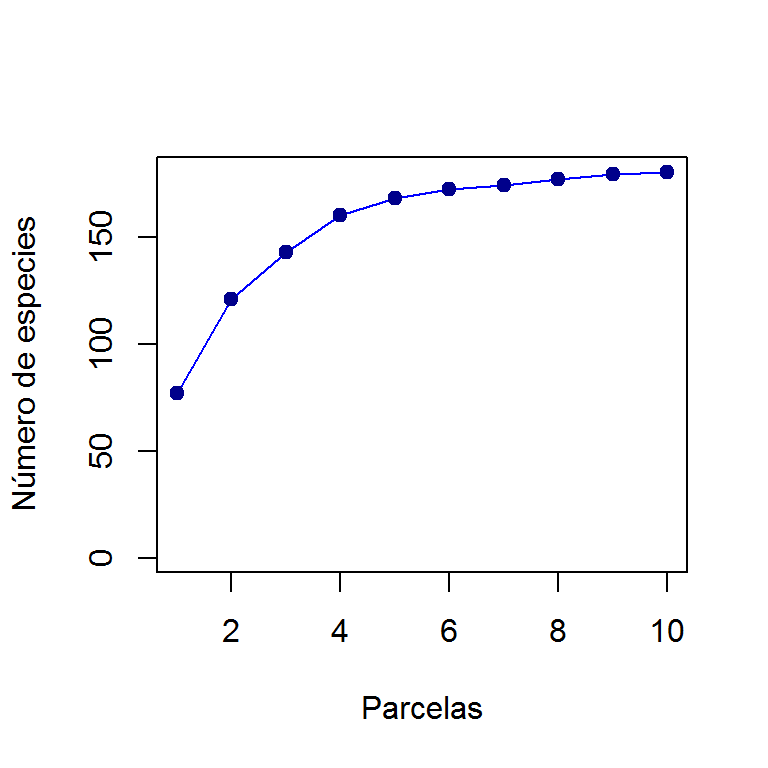
\includegraphics{Alpha-Diversidad_files/figure-latex/accum-1} 

}

\caption{Curva de acumulación de especies}\label{fig:accum}
\end{figure}

En la figura \ref{fig:accum} podemos ver como la riqueza incrementa con
el aumento del área muestreal, cada nueva muestra incluye nuevas
especies a la comunidad. Podemos observar que la curva muestra
``saltos'', alguna parcela incluye más especies nuevas que otras. La
forma de esta curva está dada por el orden en el cual las parcelas
fueron subidas por el colector. Aunque la curva de acumulación de
especies nos permite evaluar como nuestro muestreo incorpora especies y
si hemos tenido un buen muestreo, esta es muy dependiente del orden en
el cual se dispongan las muestras. Una forma más eficiente sería
aleatorizar el orden y construir una curva, este proceso es conocido
como rarefacción.

\chapter{Rarefacción}\label{rarefaccion}

La riqueza es una de las medidas más simples e intuitivas que describen
una comunidad, sin embargo, uno de los problemas del uso de esta medida
es su dependencia del tamaño muestreal (Magurran 2004), esto implica que
la riqueza (y las otras medidas de diversidad) puede verse influida por
variaciones en el esfuerzo muestreal. Aunque el diseño experimental está
pensado para estandarizar el esfuerzo muestreal, los tamaños finales
muestreales difícilmente son iguales.

\begin{quote}
Un esfuerzo de muestreo desigual puede tener impactos en las medidas de
riqueza de especies

--- (Magurran 2004)
\end{quote}

Esto representa un inconveniente, ya que muestreos en principio del
mismo tamaño, podrían capturar números significativamente diferentes de
individuos. Pensemos que una red para aves podría capturar 150
individuos en un sitio y 25 en otro. Cuan comparables serían estos datos
si sabemos que el tamaño de la muestra influye en la cantidad de
especies colectadas.

De esta manera, necesitamos separar dos conceptos distintos, la densidad
de especies de la riqueza de especies. Imaginemos dos área cualquiera
donde vamos a muestrear la vegetación, estas dos áreas únicamente se
diferencian porque en la una existe pastoreo y en la otra no. Vemos que
pasa cuando muestreamos cada una de estas comunidades.

\begin{Shaded}
\begin{Highlighting}[]
\CommentTok{#Generamos unas comunidades}
\NormalTok{pas <-}\StringTok{ }\KeywordTok{data.frame}\NormalTok{( }\DataTypeTok{sp =} \KeywordTok{paste}\NormalTok{(}\KeywordTok{rep}\NormalTok{(}\StringTok{"sp"}\NormalTok{, }\DecValTok{30}\NormalTok{), }\DecValTok{1}\NormalTok{:}\DecValTok{30}\NormalTok{, }\DataTypeTok{sep=}\StringTok{"-"}\NormalTok{), }\DataTypeTok{abun=} \KeywordTok{sample}\NormalTok{(}\DecValTok{1}\NormalTok{:}\DecValTok{12}\NormalTok{, }\DecValTok{30}\NormalTok{, }\DataTypeTok{replace=}\OtherTok{TRUE}\NormalTok{))}
\NormalTok{pas1 <-}\StringTok{ }\KeywordTok{matrix}\NormalTok{(}\DecValTok{0}\NormalTok{, }\DecValTok{40}\NormalTok{,}\DecValTok{30}\NormalTok{)}
\KeywordTok{colnames}\NormalTok{(pas1) <-}\StringTok{ }\NormalTok{pas[,}\DecValTok{1}\NormalTok{]}
\NormalTok{for(i in }\DecValTok{1}\NormalTok{:}\DecValTok{30}\NormalTok{)\{}
\NormalTok{pas1[,i] <-}\StringTok{ }\KeywordTok{c}\NormalTok{(}\KeywordTok{rep}\NormalTok{(}\DecValTok{1}\NormalTok{, pas[i,}\DecValTok{2}\NormalTok{]), }\KeywordTok{rep}\NormalTok{(}\DecValTok{0}\NormalTok{, }\DecValTok{40}\NormalTok{-pas[i,}\DecValTok{2}\NormalTok{]))}
\NormalTok{\}}
\NormalTok{pas1 <-}\StringTok{ }\NormalTok{pas1[}\KeywordTok{order}\NormalTok{(}\KeywordTok{sample}\NormalTok{(}\DecValTok{1}\NormalTok{:}\DecValTok{40}\NormalTok{, }\DecValTok{30}\NormalTok{)), ]}

\NormalTok{npas <-}\StringTok{ }\KeywordTok{data.frame}\NormalTok{( }\DataTypeTok{sp =} \KeywordTok{paste}\NormalTok{(}\KeywordTok{rep}\NormalTok{(}\StringTok{"sp"}\NormalTok{, }\DecValTok{30}\NormalTok{), }\DecValTok{1}\NormalTok{:}\DecValTok{30}\NormalTok{, }\DataTypeTok{sep=}\StringTok{"-"}\NormalTok{), }\DataTypeTok{abun=} \KeywordTok{sample}\NormalTok{(}\DecValTok{30}\NormalTok{:}\DecValTok{40}\NormalTok{, }\DecValTok{30}\NormalTok{, }\DataTypeTok{replace=}\OtherTok{TRUE}\NormalTok{))}
\NormalTok{npas1 <-}\StringTok{ }\KeywordTok{matrix}\NormalTok{(}\DecValTok{0}\NormalTok{, }\DecValTok{40}\NormalTok{,}\DecValTok{30}\NormalTok{)}
\KeywordTok{colnames}\NormalTok{(npas1) <-}\StringTok{ }\NormalTok{npas[,}\DecValTok{1}\NormalTok{]}
\NormalTok{for(i in }\DecValTok{1}\NormalTok{:}\DecValTok{30}\NormalTok{)\{}
\NormalTok{npas1[,i] <-}\StringTok{ }\KeywordTok{c}\NormalTok{(}\KeywordTok{rep}\NormalTok{(}\DecValTok{1}\NormalTok{, npas[i,}\DecValTok{2}\NormalTok{]), }\KeywordTok{rep}\NormalTok{(}\DecValTok{0}\NormalTok{, }\DecValTok{40}\NormalTok{-npas[i,}\DecValTok{2}\NormalTok{]))}
\NormalTok{\}}
\NormalTok{npas1 <-}\StringTok{ }\NormalTok{npas1[}\KeywordTok{order}\NormalTok{(}\KeywordTok{sample}\NormalTok{(}\DecValTok{1}\NormalTok{:}\DecValTok{20}\NormalTok{, }\DecValTok{20}\NormalTok{)), ]}

\CommentTok{#Ahora las muestreamos}
\NormalTok{m_pas <-}\StringTok{ }\KeywordTok{matrix}\NormalTok{(}\DecValTok{0}\NormalTok{,}\DecValTok{3}\NormalTok{,}\DecValTok{30}\NormalTok{)}
\KeywordTok{colnames}\NormalTok{(m_pas) <-}\StringTok{ }\KeywordTok{colnames}\NormalTok{(pas1)}
\NormalTok{m_pas[}\DecValTok{1}\NormalTok{,] <-}\StringTok{ }\KeywordTok{sample}\NormalTok{(pas1, }\DecValTok{30}\NormalTok{)}
\NormalTok{m_pas[}\DecValTok{2}\NormalTok{,] <-}\StringTok{ }\KeywordTok{sample}\NormalTok{(pas1, }\DecValTok{30}\NormalTok{)}
\NormalTok{m_pas[}\DecValTok{3}\NormalTok{,] <-}\StringTok{ }\KeywordTok{sample}\NormalTok{(pas1, }\DecValTok{30}\NormalTok{)}

\NormalTok{m_npas <-}\StringTok{ }\KeywordTok{matrix}\NormalTok{(}\DecValTok{0}\NormalTok{,}\DecValTok{3}\NormalTok{,}\DecValTok{30}\NormalTok{)}
\KeywordTok{colnames}\NormalTok{(m_npas) <-}\StringTok{ }\KeywordTok{colnames}\NormalTok{(pas1)}
\NormalTok{m_npas[}\DecValTok{1}\NormalTok{,] <-}\StringTok{ }\KeywordTok{sample}\NormalTok{(npas1, }\DecValTok{30}\NormalTok{)}
\NormalTok{m_npas[}\DecValTok{2}\NormalTok{,] <-}\StringTok{ }\KeywordTok{sample}\NormalTok{(npas1, }\DecValTok{30}\NormalTok{)}
\NormalTok{m_npas[}\DecValTok{3}\NormalTok{,] <-}\StringTok{ }\KeywordTok{sample}\NormalTok{(npas1, }\DecValTok{30}\NormalTok{)}

\CommentTok{#Calculamos la riqueza de las muestras}
\KeywordTok{specnumber}\NormalTok{(}\KeywordTok{colSums}\NormalTok{(m_pas)) }\CommentTok{#Pastoreado}
\end{Highlighting}
\end{Shaded}

\begin{verbatim}
## [1] 13
\end{verbatim}

\begin{Shaded}
\begin{Highlighting}[]
\KeywordTok{specnumber}\NormalTok{(}\KeywordTok{colSums}\NormalTok{(m_npas))}\CommentTok{#No Pastoreado}
\end{Highlighting}
\end{Shaded}

\begin{verbatim}
## [1] 30
\end{verbatim}

Como vemos por puro azar la diversidad es mucho mayor en las parcelas no
pastoreadas, pero realmente hay mayor diversidad? Obtengamos la
diversidad total de cada comunidad.

\begin{Shaded}
\begin{Highlighting}[]
\KeywordTok{specnumber}\NormalTok{(}\KeywordTok{colSums}\NormalTok{(pas1))}\CommentTok{#Pastoreado}
\end{Highlighting}
\end{Shaded}

\begin{verbatim}
## [1] 30
\end{verbatim}

\begin{Shaded}
\begin{Highlighting}[]
\KeywordTok{specnumber}\NormalTok{(}\KeywordTok{colSums}\NormalTok{(npas1))}\CommentTok{#No Pastoreado}
\end{Highlighting}
\end{Shaded}

\begin{verbatim}
## [1] 30
\end{verbatim}

Efectivamente la riqueza es la misma, el único problema es que en la
zona pastoreada tiene una menor abundancia lo que origina una menor
densidad de especies, sin embargo, no hay un efecto sobre la riqueza de
especies.

Algunos índices basados en la riqueza como el de Margalef y Menhinick
han sido propuestos para minimizar estos efectos, pero este ajuste ha
mostrado ser insuficiente (Magurran, 2004). Una solución más aceptada a
este problema es realizar una rarefacción, que es una forma de
remuestrear las parcelas en función de un tamaño de muestra único para
todas las parcelas.

Específicamente la rarefacción es el proceso de generación de la
relación entre el número de especies vs el número de individuos en una o
más muestras (Stevens 2009). Esta corrección por el número de individuos
nos permite la comparación directa de la riqueza de dos muestras que
inicialmente tenían diferente tamaño.

Para poder abordar estos temas utilizaremos la función \texttt{rarefy}
del paquete \emph{vegan}. La función \texttt{rarefy} arroja como
resultado la riqueza de especies esperada en un determinado tamaño de
muestra.

La rarefacción puede realizarse solamente con auténticos datos de
conteos. La función \emph{rarefy} se basa en la formulación de Hurlbert
(1971), y los errores estándar sobre Heck et al. (1975).

Hurlbert (1971) propone la rarefacción como:

\[S_n= \sum_{i=1}^S (1-q_i)\]

Donde; \(q_i= \frac{(\frac{n-x_i}{n})}{(\frac{N}{n})}\) que representa
las probabilidades de que las especies \emph{i} no ocurra en una muestra
de tamaño \emph{n}, \(x_i\) es el conteo de \emph{i} especies y
\((\frac{N}{n})\) es el coeficiente binomial o el número de formas en
las que puede elegir n de N

En otras palabras la rarefacción permite hacer una interpolación de los
datos, obteniendo una riqueza esperada en un tamaño de muestra menor al
tamaño que hemos logrado, de esta forma este proceso nos da no solamente
la riqueza sino un error estándar. Si la muestra es un vector, la
rarefacción se calculará para cada tamaño de la muestra por separado.

A continuación vamos a utilizar la función \emph{rarefy} para construir
las curvas de rarefacción basadas en individuos y en muestras.

\section{Rarefacción basada en
Individuos}\label{rarefaccion-basada-en-individuos}

Vamos a utilizar nuestros ya conocidos datos de BCI, a partir de estos
datos realizaremos un submuestreo escogiendo 10 de las 50 parcelas de
BCI, esto con el fin de simplificar el ejemplo.

Lo primero que necesitamos es obtener un vector (un objeto) con el total
de individuos de cada especie, este objeto representa la comunidad sobre
la que haremos la rarefacción y la estimación de la riqueza total.
Queremos generar una curva parecida a la de acumulación de especies pero
que nos dará una riqueza con el error estándar, para esto tenemos que
definir en qué tamaños de muestra queremos hacer la interpolación. Vamos
a realizar estos pasos en R.

\begin{Shaded}
\begin{Highlighting}[]
\CommentTok{#Usaremos los datos con los cuales construimos las curvas de acumulación}
\CommentTok{#Sumamos la abundancia de cada especie}
\NormalTok{N <-}\StringTok{ }\KeywordTok{colSums}\NormalTok{(BCI_sub) }

\CommentTok{#Hacemos un vector con los tamaños de muestra sobre los cuales haremos }
\CommentTok{#la interpolación. El dato final de este vector es el tamaño total de la }
\CommentTok{#muestra (sum(N))}
\NormalTok{subs3 <-}\StringTok{ }\KeywordTok{c}\NormalTok{(}\KeywordTok{seq}\NormalTok{(}\DecValTok{500}\NormalTok{, }\DecValTok{4000}\NormalTok{, }\DataTypeTok{by =} \DecValTok{500}\NormalTok{), }\KeywordTok{sum}\NormalTok{(N)) }

\CommentTok{#Ejecutamos la rarefacción}
\NormalTok{rar3 <-}\StringTok{ }\KeywordTok{rarefy}\NormalTok{(N, }\DataTypeTok{sample =} \NormalTok{subs3, }\DataTypeTok{se =} \NormalTok{T, }\DataTypeTok{MARG =} \DecValTok{2}\NormalTok{)}
\NormalTok{rar3}
\end{Highlighting}
\end{Shaded}

\begin{verbatim}
##           N500      N1000      N1500      N2000     N2500      N3000
## .S  106.511010 132.555792 146.508684 155.622094 162.27681 167.469582
## .se   4.615179   4.268649   3.873036   3.491962   3.09491   2.647784
##         N3500      N4000 N4276
## .S  171.69984 175.255907   177
## .se   2.09532   1.274649     0
## attr(,"Subsample")
## [1]  500 1000 1500 2000 2500 3000 3500 4000 4276
\end{verbatim}

Como vemos el objeto rar3 nos muestra la cantidad de especies que se
espera tener a diferentes tamaños de muestras, en el ejemplo desde 500
hasta 4296. En este caso en el tamaño de 500 se espera tener 108.32
especies con un error estándar de 4.63. La riqueza tiene decimales pues
es la media de la aleatorización realizada.

\section{Rarefacción basada en
muestras}\label{rarefaccion-basada-en-muestras}

Para realizar una rarefacción basada en muestras utilizaremos los
modelos de acumulación de especies de la función \texttt{specaccum} del
paquete \emph{vegan}. Utilizaremos el método ``\emph{random}'' de esta
función, que encuentra la riqueza de especies esperada para un tamaño de
muestra.

\begin{Shaded}
\begin{Highlighting}[]
\NormalTok{rand<-}\KeywordTok{specaccum}\NormalTok{(BCI_sub, }\DataTypeTok{method =} \StringTok{"random"}\NormalTok{, }\DataTypeTok{permutations=}\DecValTok{100}\NormalTok{)}
\NormalTok{rand}
\end{Highlighting}
\end{Shaded}

\begin{verbatim}
## Species Accumulation Curve
## Accumulation method: random, with 100 permutations
## Call: specaccum(comm = BCI_sub, method = "random", permutations = 100) 
## 
##                                                                    
## Sites     1.00000   2.00000   3.00000   4.00000   5.00000   6.00000
## Richness 92.57000 122.46000 137.97000 148.38000 155.91000 161.65000
## sd        6.66402   8.08593   6.61412   5.84787   5.27064   4.90593
##                                           
## Sites      7.00000   8.00000   9.00000  10
## Richness 166.26000 170.72000 174.21000 177
## sd         4.32661   3.49915   2.40914   0
\end{verbatim}

En este caso lo que vemos es que con una sola muestra tendríamos 92.55
especies, con dos parcelas tendríamos 123.9 especies, y así
sucesivamente como podemos ver aparentemente la curva tiende a
estabilizarse a partir de la parcela 7.

\section{Estimadores de Riqueza}\label{estimadores-de-riqueza}

Como vemos el efecto que tiene el esfuerzo de muestreo sobre la riqueza
hace que medirla de forma exacta y precisa sea un tanto complejo. La
comparación de la riqueza debería realizársela sólo a partir de
inventarios completos (que han llegado a la asíntota de la curva de
acumulación de especies), lo que generalmente es muy difícil de lograr
con unos recursos limitados (ej. Longino et al 2002 muestra que después
de 30 años de muestreo de hormigas en la estación La Selva en Costa
Rica, no se ha logrado alcanzar la asíntota). Una buena opción para
determinar la riqueza de una comunidad consiste en estimar el número de
especies a partir de un muestreo previo.

\begin{quote}
Los estimadores de riqueza pueden ser paramétricos y no paramétricos
\end{quote}

Muchos métodos de estimas de la riqueza han sido propuestos, pero las
aproximaciones más utilizadas en ecología son mediante métodos
paramétricos y no paramétricos (Colwell \& Coddington, 1994). Los
métodos paramétricos estiman el número de especies ajustando las
abundancias de las especies a modelos de distribución paramétrica
(series logarítmica, log-normal, o Poisson log-normal). En el caso de
las aproximaciones no paramétricas se basan en el estudio de las
especies raras y permiten estimar el número de nuevas especies a partir
de las relaciones de abundancia o incidencia de las especies ya
detectadas en el muestreo (González-Oreja et al. 2010).

Para estimar el número total de especies (riqueza asintótica)
utilizaremos estimadores no-paramétricos. En primer lugar, utilizamos un
estimador de riqueza basado en la abundancia el \emph{ACE}, esta
estimación la podemos hacer con la función \texttt{estimateR} que se
encuentra en el paquete \emph{vegan}. Además, utilizamos un estimador
basado en la frecuencia de especies, Chao 2. Este estimador necesita
datos de presencia/ausencia y múltiples parcelas de muestreo. Para esto
utilizamos la función \texttt{specpool}.

\begin{Shaded}
\begin{Highlighting}[]
\CommentTok{#Utilizaremos el valor obtenido de la suma de todas las especies que obtuvimos previamente}
\NormalTok{ace <-}\StringTok{ }\KeywordTok{estimateR}\NormalTok{(N)}

\CommentTok{#Podemos aplicar directamente sobre nuestra matriz y nos arroja un solo dato}
\NormalTok{chaoF <-}\StringTok{ }\KeywordTok{specpool}\NormalTok{(BCI_sub) }
\NormalTok{ace; chaoF}
\end{Highlighting}
\end{Shaded}

\begin{verbatim}
##      S.obs    S.chao1   se.chao1      S.ACE     se.ACE 
## 177.000000 197.312500  10.512240 193.287756   6.899095
\end{verbatim}

\begin{verbatim}
##     Species  chao chao.se jack1 jack1.se    jack2     boot  boot.se  n
## All     177 193.8     8.4 202.2 10.69953 209.6667 189.6454 6.595226 10
\end{verbatim}

Como vemos las dos funciones nos dan varios índices no únicamente el ACE
y el Chao2. Según lo que creamos conveniente podemos utilizar cualquiera
de ellos. El estimador ACE es bastante conservador y nos da una riqueza
esperada de 196.08 con un error estándar de 6.83, mientras que Chao (de
la función specpool) nos da una riqueza de 197.64 con una desviación de
6.63. En este caso el estimador Jacknife2 nos da la más alta riqueza con
213 especies.

\section{Graficando los resultados}\label{graficando-los-resultados}

Ahora, graficamos las curvas de rarefacción basada en individuos y en
muestras con su desviación estándar en los distintos tamaños de muestra
escogidos, adicionalmente incluiremos los estimadores de riqueza y la
riqueza total en las 50 ha del BCI.

\begin{Shaded}
\begin{Highlighting}[]
\KeywordTok{par}\NormalTok{(}\DataTypeTok{mar=}\KeywordTok{c}\NormalTok{(}\DecValTok{6}\NormalTok{,}\DecValTok{4}\NormalTok{,}\DecValTok{1}\NormalTok{,}\DecValTok{1}\NormalTok{))}

\CommentTok{#construimos el gráfico de rarefacción basada en individuos}
\KeywordTok{plot}\NormalTok{(subs3, rar3[}\DecValTok{1}\NormalTok{, ], }\DataTypeTok{ylab =} \StringTok{"Riqueza de especies"}\NormalTok{, }
          \DataTypeTok{axes =} \OtherTok{FALSE}\NormalTok{, }\DataTypeTok{xlab =} \StringTok{""}\NormalTok{, }\DataTypeTok{cex.lab=}\FloatTok{0.8}\NormalTok{, }
        \DataTypeTok{type =} \StringTok{"l"}\NormalTok{, }\DataTypeTok{ylim =} \KeywordTok{c}\NormalTok{(}\DecValTok{50}\NormalTok{, }\DecValTok{260}\NormalTok{), }\DataTypeTok{xlim =} \KeywordTok{c}\NormalTok{(}\DecValTok{500}\NormalTok{, }\DecValTok{7000}\NormalTok{), }\DataTypeTok{lwd=}\FloatTok{1.8}\NormalTok{)}
\KeywordTok{points}\NormalTok{(subs3,rar3[}\DecValTok{1}\NormalTok{, ], }\DataTypeTok{pch=}\DecValTok{19}\NormalTok{)}

\CommentTok{#Graficamos la desviación estándar.}
\KeywordTok{segments}\NormalTok{(subs3, rar3[}\DecValTok{1}\NormalTok{, ] +}\StringTok{ }\DecValTok{2} \NormalTok{*}\StringTok{ }\NormalTok{rar3[}\DecValTok{2}\NormalTok{, ], }
         \NormalTok{subs3, rar3[}\DecValTok{1}\NormalTok{, ] -}\StringTok{ }\DecValTok{2} \NormalTok{*}\StringTok{ }\NormalTok{rar3[}\DecValTok{2}\NormalTok{, ])}

\CommentTok{#Graficamos los ejes}
\KeywordTok{axis}\NormalTok{(}\DecValTok{1}\NormalTok{, }\DataTypeTok{at =} \DecValTok{1}\NormalTok{:}\DecValTok{5} \NormalTok{*}\StringTok{ }\DecValTok{1000}\NormalTok{, }\DataTypeTok{cex.axis=}\FloatTok{0.7}\NormalTok{,}\DataTypeTok{mgp=}\KeywordTok{c}\NormalTok{(}\DecValTok{3}\NormalTok{, }\FloatTok{0.2}\NormalTok{, }\DecValTok{0}\NormalTok{)) }
\KeywordTok{axis}\NormalTok{(}\DecValTok{2}\NormalTok{, }\DataTypeTok{cex.axis=}\FloatTok{0.7}\NormalTok{) }

\CommentTok{#la caja}
\KeywordTok{box}\NormalTok{() }

\CommentTok{#Sobreponemos la curva de rarefacción basada en muestras}
\KeywordTok{par}\NormalTok{(}\DataTypeTok{new=}\NormalTok{T)}
\CommentTok{#Hacemos un vector con el número de parcelas}
\NormalTok{x<-}\StringTok{ }\DecValTok{1}\NormalTok{:}\DecValTok{10}

\CommentTok{#Graficamos la curva}
\KeywordTok{plot}\NormalTok{(x, rand$richness, }\DataTypeTok{type=}\StringTok{"l"}\NormalTok{, }\DataTypeTok{col=}\StringTok{"red"}\NormalTok{,}\DataTypeTok{ylab=}\StringTok{""}\NormalTok{, }\DataTypeTok{xlab=}\StringTok{""}\NormalTok{, }
     \DataTypeTok{axes=}\OtherTok{FALSE}\NormalTok{, }\DataTypeTok{xlim=}\KeywordTok{c}\NormalTok{(}\DecValTok{1}\NormalTok{,}\DecValTok{15}\NormalTok{), }\DataTypeTok{ylim =} \KeywordTok{c}\NormalTok{(}\DecValTok{50}\NormalTok{, }\DecValTok{260}\NormalTok{), }\DataTypeTok{lwd=}\FloatTok{1.8}\NormalTok{)}
\KeywordTok{points}\NormalTok{(rand$richness, }\DataTypeTok{pch=}\DecValTok{19}\NormalTok{, }\DataTypeTok{col=}\StringTok{"darkred"}\NormalTok{)}
\KeywordTok{segments}\NormalTok{(x, rand$richness +}\StringTok{ }\DecValTok{2} \NormalTok{*}\StringTok{ }\NormalTok{rand$sd, x, rand$richness -}\StringTok{ }\DecValTok{2} \NormalTok{*}\StringTok{ }\NormalTok{rand$sd, }\DataTypeTok{col=}\StringTok{"red"}\NormalTok{)}

\CommentTok{#Graficamos la curva de acumulación}
\KeywordTok{par}\NormalTok{(}\DataTypeTok{new=}\NormalTok{T)}
\KeywordTok{plot}\NormalTok{(col, }\DataTypeTok{xlab=}\StringTok{""}\NormalTok{, }\DataTypeTok{ylab=}\StringTok{""}\NormalTok{, }\DataTypeTok{col=}\StringTok{"blue"}\NormalTok{, }\DataTypeTok{axes=}\OtherTok{FALSE}\NormalTok{, }\DataTypeTok{xlim=}\KeywordTok{c}\NormalTok{(}\DecValTok{1}\NormalTok{,}\DecValTok{15}\NormalTok{), }
     \DataTypeTok{ylim =} \KeywordTok{c}\NormalTok{(}\DecValTok{50}\NormalTok{, }\DecValTok{260}\NormalTok{), }\DataTypeTok{lwd=}\FloatTok{1.8}\NormalTok{)}
\KeywordTok{points}\NormalTok{(col$richness, }\DataTypeTok{pch=}\DecValTok{19}\NormalTok{, }\DataTypeTok{col=}\StringTok{"darkblue"}\NormalTok{)}

\KeywordTok{axis}\NormalTok{(}\DecValTok{1}\NormalTok{, }\DataTypeTok{at=}\DecValTok{1}\NormalTok{:}\DecValTok{10}\NormalTok{, }\DataTypeTok{cex.axis=}\FloatTok{0.7}\NormalTok{, }\DataTypeTok{line =}\DecValTok{3}\NormalTok{, }\DataTypeTok{mgp=}\KeywordTok{c}\NormalTok{(}\DecValTok{3}\NormalTok{, }\FloatTok{0.2}\NormalTok{, }\DecValTok{0}\NormalTok{)) }

\KeywordTok{mtext}\NormalTok{(}\StringTok{"No. Individuos"}\NormalTok{, }\DataTypeTok{side=}\DecValTok{1}\NormalTok{, }\DataTypeTok{line=}\FloatTok{1.3}\NormalTok{, }\DataTypeTok{cex=}\FloatTok{0.8}\NormalTok{, }\DataTypeTok{at=}\DecValTok{6}\NormalTok{)}
\KeywordTok{mtext}\NormalTok{(}\StringTok{"No. Parcelas"}\NormalTok{, }\DataTypeTok{side=}\DecValTok{1}\NormalTok{, }\DataTypeTok{line=}\DecValTok{4}\NormalTok{, }\DataTypeTok{cex=}\FloatTok{0.8}\NormalTok{, }\DataTypeTok{at=}\DecValTok{6}\NormalTok{)}

\KeywordTok{legend}\NormalTok{(}\DecValTok{1}\NormalTok{, }\DecValTok{250}\NormalTok{, }\KeywordTok{c}\NormalTok{(}\StringTok{"Rarefacción - Muestras"}\NormalTok{, }\StringTok{"Curva de acumulación"}\NormalTok{,}
                 \StringTok{"Rarefacción - Individuos"}\NormalTok{), }\DataTypeTok{lty=}\KeywordTok{c}\NormalTok{(}\DecValTok{1}\NormalTok{,}\DecValTok{1}\NormalTok{,}\DecValTok{1}\NormalTok{), }\DataTypeTok{pch=}\DecValTok{19}\NormalTok{,}
       \DataTypeTok{cex=}\FloatTok{0.7}\NormalTok{, }\DataTypeTok{col =} \KeywordTok{c}\NormalTok{(}\StringTok{"red"}\NormalTok{, }\StringTok{"blue"}\NormalTok{, }\StringTok{"black"}\NormalTok{))}

\CommentTok{#Incluimos el estimador de riqueza ACE}
\KeywordTok{points}\NormalTok{(}\DecValTok{11}\NormalTok{,ace[}\StringTok{"S.ACE"}\NormalTok{], }\DataTypeTok{pch=}\DecValTok{19}\NormalTok{)}
\KeywordTok{segments}\NormalTok{(}\DecValTok{11}\NormalTok{, ace[}\StringTok{"S.ACE"}\NormalTok{] -}\StringTok{ }\DecValTok{2} \NormalTok{*}\StringTok{ }\NormalTok{ace[}\StringTok{"se.ACE"}\NormalTok{], }
         \DecValTok{11}\NormalTok{, ace[}\StringTok{"S.ACE"}\NormalTok{] +}\StringTok{ }\DecValTok{2} \NormalTok{*}\StringTok{ }\NormalTok{ace[}\StringTok{"se.ACE"}\NormalTok{], }\DataTypeTok{lwd =} \DecValTok{3}\NormalTok{) }

\KeywordTok{text}\NormalTok{(}\DecValTok{11}\NormalTok{, }\DecValTok{160}\NormalTok{, }\StringTok{"Estimador ACE"}\NormalTok{, }\DataTypeTok{srt =} \DecValTok{90}\NormalTok{, }\DataTypeTok{adj =} \KeywordTok{c}\NormalTok{(}\DecValTok{1}\NormalTok{, +}\StringTok{ }\FloatTok{0.5}\NormalTok{), }\DataTypeTok{cex=}\FloatTok{0.7}\NormalTok{)}

\CommentTok{#Incluimos el estimador de riqueza Chao2}
\KeywordTok{points}\NormalTok{(}\DecValTok{12}\NormalTok{,chaoF[}\DecValTok{1}\NormalTok{, }\StringTok{"chao"}\NormalTok{], }\DataTypeTok{pch=}\DecValTok{19}\NormalTok{, }\DataTypeTok{col=}\StringTok{"grey"}\NormalTok{)}
\KeywordTok{segments}\NormalTok{(}\DecValTok{12}\NormalTok{, chaoF[}\DecValTok{1}\NormalTok{, }\StringTok{"chao"}\NormalTok{] -}\StringTok{ }\DecValTok{2} \NormalTok{*}\StringTok{ }\NormalTok{chaoF[}\DecValTok{1}\NormalTok{, }
                \StringTok{"chao.se"}\NormalTok{], }\DecValTok{12}\NormalTok{, chaoF[}\DecValTok{1}\NormalTok{, }\StringTok{"chao"}\NormalTok{] +}\StringTok{ }\DecValTok{2} \NormalTok{*}\StringTok{ }\NormalTok{chaoF[}\DecValTok{1}\NormalTok{,}
                \StringTok{"chao.se"}\NormalTok{], }\DataTypeTok{lwd =} \DecValTok{3}\NormalTok{, }\DataTypeTok{col =} \StringTok{"grey"}\NormalTok{) }
\KeywordTok{text}\NormalTok{(}\DecValTok{12}\NormalTok{, }\DecValTok{160}\NormalTok{, }\StringTok{"Estimador Chao2"}\NormalTok{, }\DataTypeTok{srt =} \DecValTok{90}\NormalTok{, }\DataTypeTok{adj =} \KeywordTok{c}\NormalTok{(}\DecValTok{1}\NormalTok{, +}\StringTok{ }\FloatTok{0.5}\NormalTok{), }\DataTypeTok{cex=}\FloatTok{0.7}\NormalTok{)}

\CommentTok{#La riqueza total de la parcela de 50ha del BCI}

\KeywordTok{points}\NormalTok{(}\DecValTok{13}\NormalTok{, }\KeywordTok{dim}\NormalTok{(BCI)[}\DecValTok{2}\NormalTok{], }\DataTypeTok{pch =} \DecValTok{19}\NormalTok{, }\DataTypeTok{cex =} \DecValTok{1}\NormalTok{) }
\KeywordTok{text}\NormalTok{(}\DecValTok{13}\NormalTok{, }\DecValTok{160}\NormalTok{, }\StringTok{"Riqueza  en 50 ha del BCI"}\NormalTok{,}
     \DataTypeTok{srt =} \DecValTok{90}\NormalTok{, }\DataTypeTok{adj =} \KeywordTok{c}\NormalTok{(}\DecValTok{1}\NormalTok{, }\FloatTok{0.5}\NormalTok{), }\DataTypeTok{cex=}\FloatTok{0.7}\NormalTok{)}
\KeywordTok{text}\NormalTok{(}\DecValTok{13}\NormalTok{, }\DecValTok{232}\NormalTok{, }\KeywordTok{dim}\NormalTok{(BCI)[}\DecValTok{2}\NormalTok{], }\DataTypeTok{cex=}\FloatTok{0.6}\NormalTok{)}
\end{Highlighting}
\end{Shaded}

\begin{figure}[htbp]
\centering
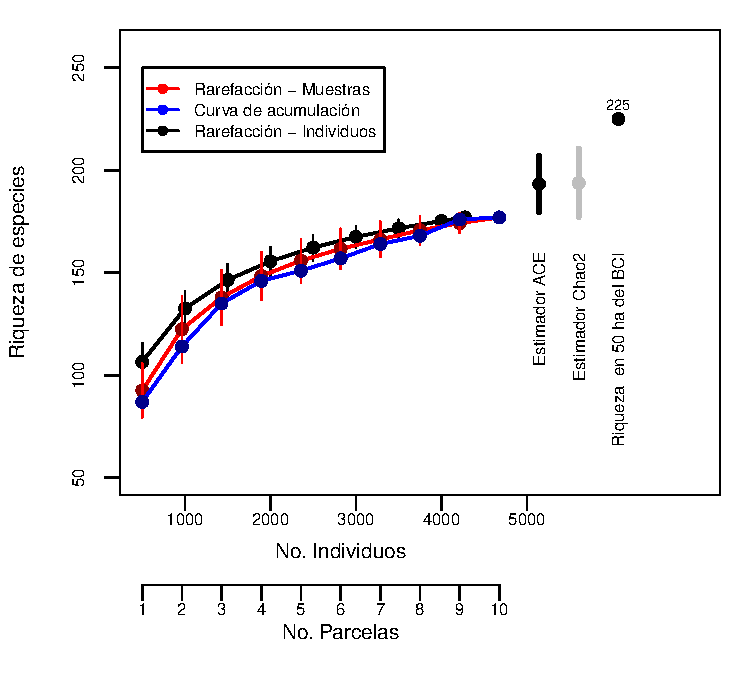
\includegraphics{Alpha-Diversidad_files/figure-latex/rar-1.pdf}
\caption{\label{fig:rar}Curvas de rarefacción basada en individuos y en
muestras de 10 parcelas al azar del BCI. Estimadores de riqueza (ACE) y
Chao2 y riqueza total obtenida en las 50 ha del BCI.}
\end{figure}

En la figura \ref{fig:rar} podemos ver que nuestro muestreo es aceptable
y que aunque no hemos capturado toda la riqueza del área los estimadores
que utilizamos son aceptables. Es posible que en este caso la riqueza de
jacknife sea un mejor estimador. Pero recuerden que normalmente cuando
hacemos un muestreo no tenemos el valor de riqueza total, por lo que no
podemos saber cuan alejados estamos de la realidad.

\chapter{Comparando muestras}\label{comparando-muestras}

Placeholder

\chapter{Medidas de Diversidad}\label{medidas-de-diversidad}

Placeholder

\subsection{Índice de Simpson}\label{indice-de-simpson}

\chapter{Ejercicio Práctico}\label{ejercicio-practico}

Placeholder

\bibliography{book.bib}


\end{document}
